\begin{frame}{Proof Systems}

    \begin{definition}[Cook, Reckhow 79]
        Proof system for $L \Leftrightarrow$ poly-time algorithm
        $\Pi\colon \{0, 1\}^* \times \{0, 1\}^* \rightarrow \{0, 1\}$:
        \begin{itemize}
            \item (completeness) $x \in L \Rightarrow \exists w ~ \Pi(x, w) = 1$;
            \item (soundness) $\exists w ~ \Pi(x, w) = 1 \Rightarrow x \in L$.
        \end{itemize}
    \end{definition}

    \deftext{Resolution}: proof of $\varphi \coloneqq \bigwedge\limits_{i} C_i$ is a sequence of clauses
    $(D_1, D_2, D_3, \dots, D_{\ell})$:
    \pause
    
    \begin{minipage}{0.3\linewidth}
        \begin{itemize}
            \item $D_i \in \{C_i\}$;
                \pause
            \item $\frac{A \lor x ~~~~~ B \lor \bar{x}}{A \lor B}$, $D_i \coloneqq A \lor B$;
                \pause
            \item $D_{\ell} = \emptyset$.
        \end{itemize}
    \end{minipage}
    \pause
    \begin{minipage}{0.68\linewidth}
        \centering
        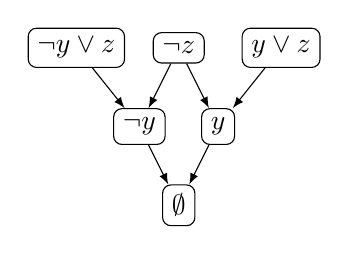
\begin{tikzpicture}[>=latex]
    \node[rectangle, rounded corners = 3pt, draw] (a) at (-1.3, 2)
        {$\neg y \lor z$};
    \node[rectangle, rounded corners = 3pt, draw] (a2) at (1.3, 2)
        {$y \lor z$};
    \node[rectangle, rounded corners = 3pt, draw] (b) at (0, 2)
        {$\neg z$};
    \node[rectangle, rounded corners = 3pt, draw] (c) at (-0.5, 1)
        {$\neg y$};
    \node[rectangle, rounded corners = 3pt, draw] (d) at (0.5, 1)
       {$y$};
    \node[rectangle, rounded corners = 3pt, draw] (e) at (0, 0)
        {$\emptyset$};

    \draw[->] (a) -- (c);
    \draw[->] (a2) -- (d);
    \draw[->] (b) -- (c);
    \draw[->] (b) -- (d);
    \draw[->] (c) -- (e);
    \draw[->] (d) -- (e);
\end{tikzpicture}
    \end{minipage}


    \pause
    \vspace{0.3cm}

    \deftext{Cutting Planes}: proof is a sequence of inequalities over $\mathbb{Z}$
    $(p_1 \ge 0, p_2 \ge 0, p_3 \ge 0, \dots, p_{\ell} \ge 0)$:
    \begin{itemize}
        \item $p_i$ is an encoding of $C \in \varphi$, $x_k \ge 0$ or $-x_k + 1 \ge 0$;
        \item $\frac{p_i ~~~~~ p_j}{p_k}$,  $(p_i \ge 0) \land (p_j \ge 0)$ imply $(p_k \ge 0)$
            \alert{over $\mathbb{Z}^n$};
        \item $p_{\ell} = 1$.
    \end{itemize}
\end{frame}

\begin{frame}{Lower bounds in proof complexity}

    
\tikzset{
    vert/.style = {
        draw,
        ellipse
    },
    tikzart-fire/.pic = {
        \draw[fill = red!60] (0, 0) .. controls (0.3, 0) and (0.6, 0.1) .. (0.7, 0.3)
            .. controls (0.8, 0.5) and (0.85, 0.6) .. (0.8, 0.9)
            .. controls (0.75, 1.1) and (0.7, 1.2) .. (0.6, 1.4)
            .. controls (0.65, 1.2) and (0.6, 1.05) .. (0.5, 0.9)
            .. controls (0.5, 1.2) and (0.2, 1.3) .. (0.1, 1.6)
            .. controls (0.05, 1.75) and (0.1, 2) .. (0.2, 2.1)
            .. controls (-0.1, 2) and (-0.2, 1.85) .. (-0.3, 1.7)
            .. controls (-0.4, 1.5) and (-0.45, 1.3) .. (-0.4, 1.1)
            .. controls (-0.5, 1.2) and (-0.51, 1.4) .. (-0.5, 1.5)
            .. controls (-0.75, 1.2) and (-0.8, 0.7) .. (-0.7, 0.5)
            .. controls (-0.6, 0.28) and (-0.4, 0) .. (0, 0);
            \fill[white] (0, 0) .. controls (0.3, 0) and (0.52, 0.34) .. (0.37, 0.61)
            .. controls (0.4, 0.54) and (0.32, 0.32) .. (0.25, 0.25)
            .. controls (0.3, 0.35) and (0.25, 0.5) .. (0.2, 0.6)
            .. controls (0.1, 0.8) and (-0.05, 1) .. (0, 1.2)
            .. controls (-0.32, 1) and (-0.3, 0.72) .. (-0.2, 0.47)
            .. controls (-0.3, 0.51) and (-0.31, 0.6) .. (-0.33, 0.7)
            .. controls (-0.4, 0.6) and (-0.4, 0.5) .. (-0.4, 0.4)
            .. controls (-0.35, 0.18) and (-0.2, 0) .. (0, 0);
    },
    semisim/.style = {
        ->,
        blue,
        dashed,
        decorate,
        decoration = {
            snake,
            amplitude = 0.5,
            segment length = 2
        }
    },        
}


    
\begin{tikzpicture}[xscale = 1.3, xshift = -1]
    \node[vert] (res) at (1, 0) {$\Res$};
    \node[vert] (ns) at (-3, 0) {$\NS$};
    \node[vert] (cp) at (3, 1) {$\CP$};
    \node[vert] (resk) at (1.2, 1.4) {$\Res(k)$};
    \node[vert] (acf) at (1.3, 2.4) {$\AC_0$-Frege};
    \node[vert] (resl) at (-1.3, 2.7) {$\ResL$};
    \node[vert] (acfp) at (0.5, 3.8) {$\AC_0[p]$-Frege};
    \node[vert] (fre) at (0.5, 5) {Frege};
    \node[vert] (ips) at (-2, 6) {$\PrSys{IPS}$};
    \node[vert] (pcr) at (-2.8, 1.9) {$\PCR[]$};
    \node[vert] (sos) at (-4, 2.5) {$\SOS$};
    
    \node[vert] (cps) at (-4, 6.5) {$\PrSys{CPS}$};

    

    \draw[->, semisim] (pcr) -- (sos);
    \draw[->] (res) -- (cp);
    \draw[->] (cp) to[out = 90, in = -20] (fre);
    \draw[->] (res) -- (resl);
    \draw[->] (res) -- (resk);
    \draw[->] (resk) -- (acf);
    \draw[->] (res) to[out = 138, in = -30] (pcr);
    \draw[->] (ns) -- (pcr);
    \draw[->] (resl) -- (acfp);
    \draw[->] (acf) -- (acfp);
    \draw[->] (acfp) -- (fre);
    \draw[->] (fre) -- (ips);
    \draw[->, semisim] (ips) -- (cps);

    \draw[->] (pcr) -- (ips);
    \draw[->] (sos) -- (cps);

    \node at (0, 6.9) {};
    

    \begin{scope}[on background layer]
        \draw[ultra thick, fill = black!5] (-4, -1) to[out = 110, in = 220] (-4.4, 3)
            to[out = 40, in = 180] (-1, 2) to[out = 0, in = 125] (2.3, 3) to[out = -55, in = 90]
            (1.5, -1);
    \end{scope}
    \node[blue] at (-1.5, 0.95) {Restriction};


    \begin{scope}[on background layer]
        \fill[orange!5] (-4, -1) to[out = 90, in = 180] (-2.3, 0.75) to[out = 0, in = 180] (0.5, 0.7)
            to[out = 0, in = 200] (3.5, 2) -- (3.5, -1) -- cycle;
        \draw[ultra thick, orange] (-4, -1) to[out = 90, in = 180] (-2.3, 0.75) to[out = 0, in = 180]
            (0.5, 0.7) to[out = 0, in = 200] (3.5, 2);
        \draw[ultra thick] (-4, -1) to[out = 110, in = 220] (-4.4, 3) to[out = 40, in = 180] (-1, 2)
            to[out = 0, in = 125] (2.3, 3) to[out = -55, in = 90] (1.5, -1);
    \end{scope}
    \node[blue] at (0, -0.7) {Mon. Interpolation};
\end{tikzpicture}
    
\end{frame}

\begin{frame}{Hard formulas for all proof systems}

    \begin{itemize}
        \item If $\varphi$ is unsatisfiable then there is a ``proof'' of unsatisfiability.
            \pause
            \begin{itemize}
                \item \alert{And we can realize it in some proof system...}
            \end{itemize}
            \pause
        \item Distribution on formulas?
            \pause
            \begin{itemize}
                \item Fine. Counting argument do not work in proof complexity.
            \end{itemize}            
    \end{itemize}

    \pause

    \vspace{1cm}
    \begin{itemize}
        \item Random $\Delta$-CNF formulas
        \item Clique formulas
        \item Pseudorandom generator formulas
    \end{itemize}
\end{frame}


\begin{frame}{Random $\Delta$-CNF}

    \begin{minipage}{0.38\linewidth}
        \centering
        \begin{tikzpicture}[>=latex]

    \foreach \i in {1, 2, ..., 6}{
        \node[draw, circle, fill = LEIblue!40, inner sep = 0pt, minimum size = 5pt]
            (a\i) at (0, -0.7 * \i) {};
    }

    \foreach \i in {1, 2, ..., 4}{
        \node[draw, circle, fill = LEIblue!40, inner sep = 0pt, minimum size = 5pt]
            (b\i) at (1.5, {-0.7 * (\i + 1)}) {};
    }

    \node[below = 8pt] at (a6) {$m$};
    \node[below = 8pt] at (b4) {$n$};
    
    \draw (a4) -- (b2);
    \draw (a4) -- (b3);
    \draw (a4) -- (b4);

    \node[right = 3pt] at (b2) {$x_1$};
    \node[right = 3pt] at (b4) {$x_2$};
    \node[right = 3pt] at (b3) {$x_3$};
\end{tikzpicture}
    \end{minipage}
    \begin{minipage}{0.58\linewidth}
        \begin{itemize}
            \item $m$ clauses;
            \item $n$ variables;
            \item $\Delta$ neighbours: $\binom{n}{\Delta}$ possibilities;
            \item negations (uniformly at random);
            \item $\mathfrak{D} \coloneqq \frac{m}{n}$ clause density.
        \end{itemize}
    \end{minipage}

    \pause
    \begin{itemize}
        \item $\mathfrak{D} > c_{\Delta} 2^{\Delta} \Rightarrow$ formula is unsat whp;
            \pause
        \item Fiege's conjecture: $\mathfrak{D} = \bigO{1} \Rightarrow$ no poly-time algorithm may
            ``prove'' unsatisfiability of random $\bigO{1}$-CNF.
            \begin{itemize}
                \item Non-approximability of many problems.
            \end{itemize}
    \end{itemize}

\end{frame}




\begin{frame}{Lower bounds in proof complexity}

    \input{pics/hier-rand.tex}
\end{frame}